\noindent FORWARD is an extensive project that integrates both software and hardware. The following section outlines the development milestones this team is complying to, as well as the allocated budget. At the time of writing this, many of the components have already been ordered, and so section \ref{sec:budget} provides an analysis of how the team is saving money or also being required to spend more. Mainly, the cost of surface mount components for the printed circuit design was somewhat overlooked during the development of the budget, but it should not be a problem due to saving money on the sensors.\\

\subsection{Project Milestones}
\noindent The figures below show various project milestones with their estimated start and end dates. The duration is given in days. There is also a Gantt chart generated by this data. The paper should be incrementally completed throughout the first semester, progressing towards a subsystem demo before an official full system prototype is made on a breadboard. After that is done, the printed circuit board will be ordered and the entirety of the second semester will be dedicated to integration and final testing and assembly. \\

\begin{figure}[H]
	\centering
	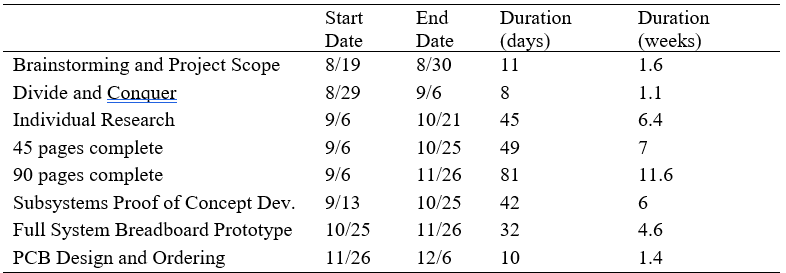
\includegraphics[width=\textwidth]{./Images/SD1mile.png}
	\caption{\label{fig:SD1mile}Senior Design I Milestones}
\end{figure}

\begin{figure}[H]
	\centering
	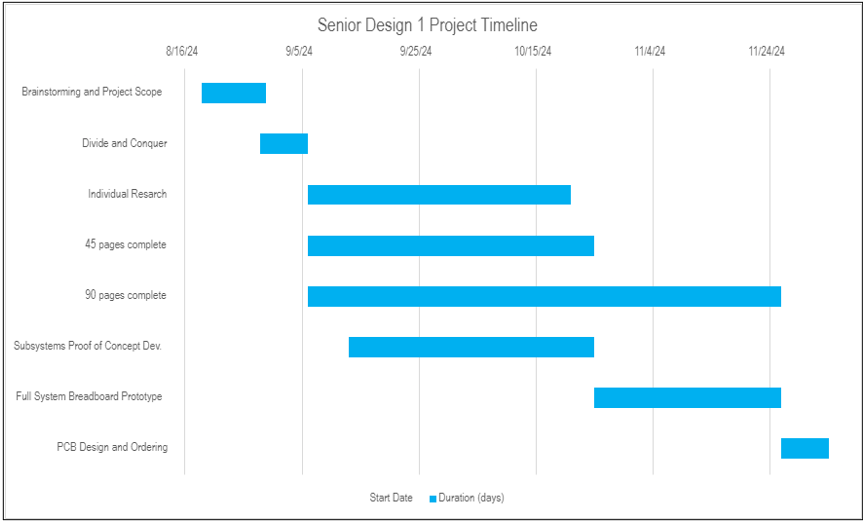
\includegraphics[width=\textwidth]{./Images/SD1gantt.png}
	\caption{\label{fig:SD1gantt}Senior Design I Gantt Chart}
\end{figure}

\noindent Senior Design II takes place during the second semester of the project, and is mainly dedicated to system integration and testing. There is a time allotted for PCB reordering, assuming that there might be problems the first time around. Much of the time will also be spent marketing and presenting the results of the project, and showcasing the hardware and software capabilities within the engineering department here at UCF.\\

\begin{figure}[H]
	\centering
	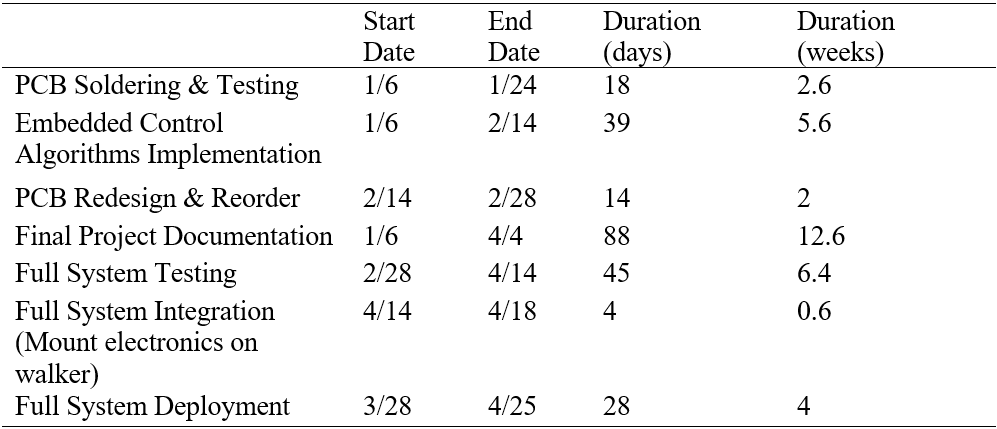
\includegraphics[width=\textwidth]{./Images/SD2mile.png}
	\caption{\label{fig:SD2mile}Senior Design II Milestones}
\end{figure}

\begin{figure}[H]
	\centering
	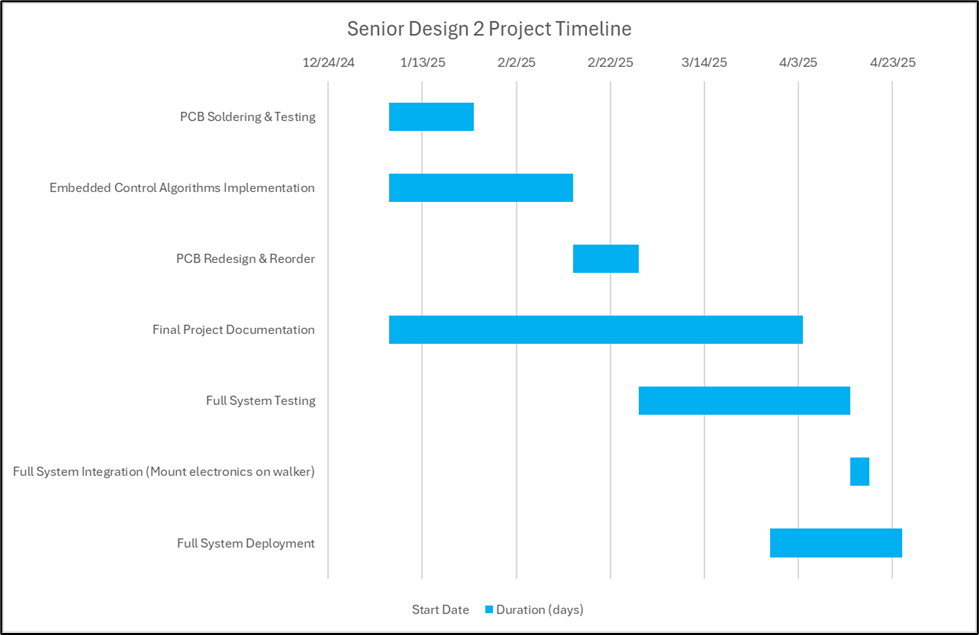
\includegraphics[width=\textwidth]{./Images/SD2gantt.png}
	\caption{\label{fig:SD2gantt}Senior Design II Gantt Chart}
\end{figure}